\newpage
\section{Ομαδοποίηση}
\subsection{Εισαγωγή στην ομαδοποίηση}
Η ενότητα αυτή αφορά τους αλγορίθμους ομαδοποίησης(\textlatin{clustering}). Η δουλειά των
αλγορίθμων αυτών είναι να χωρίσουν το σύνολο των δεδομένων σε ομάδες τέτοιες ώστε τα δεδομένα μιας
ομάδας να εμφανίζουν περισσότερες ομοιότητες μεταξύ τους από ότι με τα δεδομένα των άλλων ομάδων.
Αυτός είναι και ο βασικός στόχος της διερευνητικής και στατιστικής ανάλυσης και χρησιμοποιείται
για\cite{wikicl}:
\begin{itemize}
    \item Αναγνώριση προτύπων
    \item Ανάλυση εικόνων
    \item Εξαγωγή πληροφορίας
    \item Συμπίεση δεδομένων
    \item Γραφικά υπολογιστών
    \item Μηχανική μάθηση
\end{itemize}
\begin{figure}[H]
    \centering
    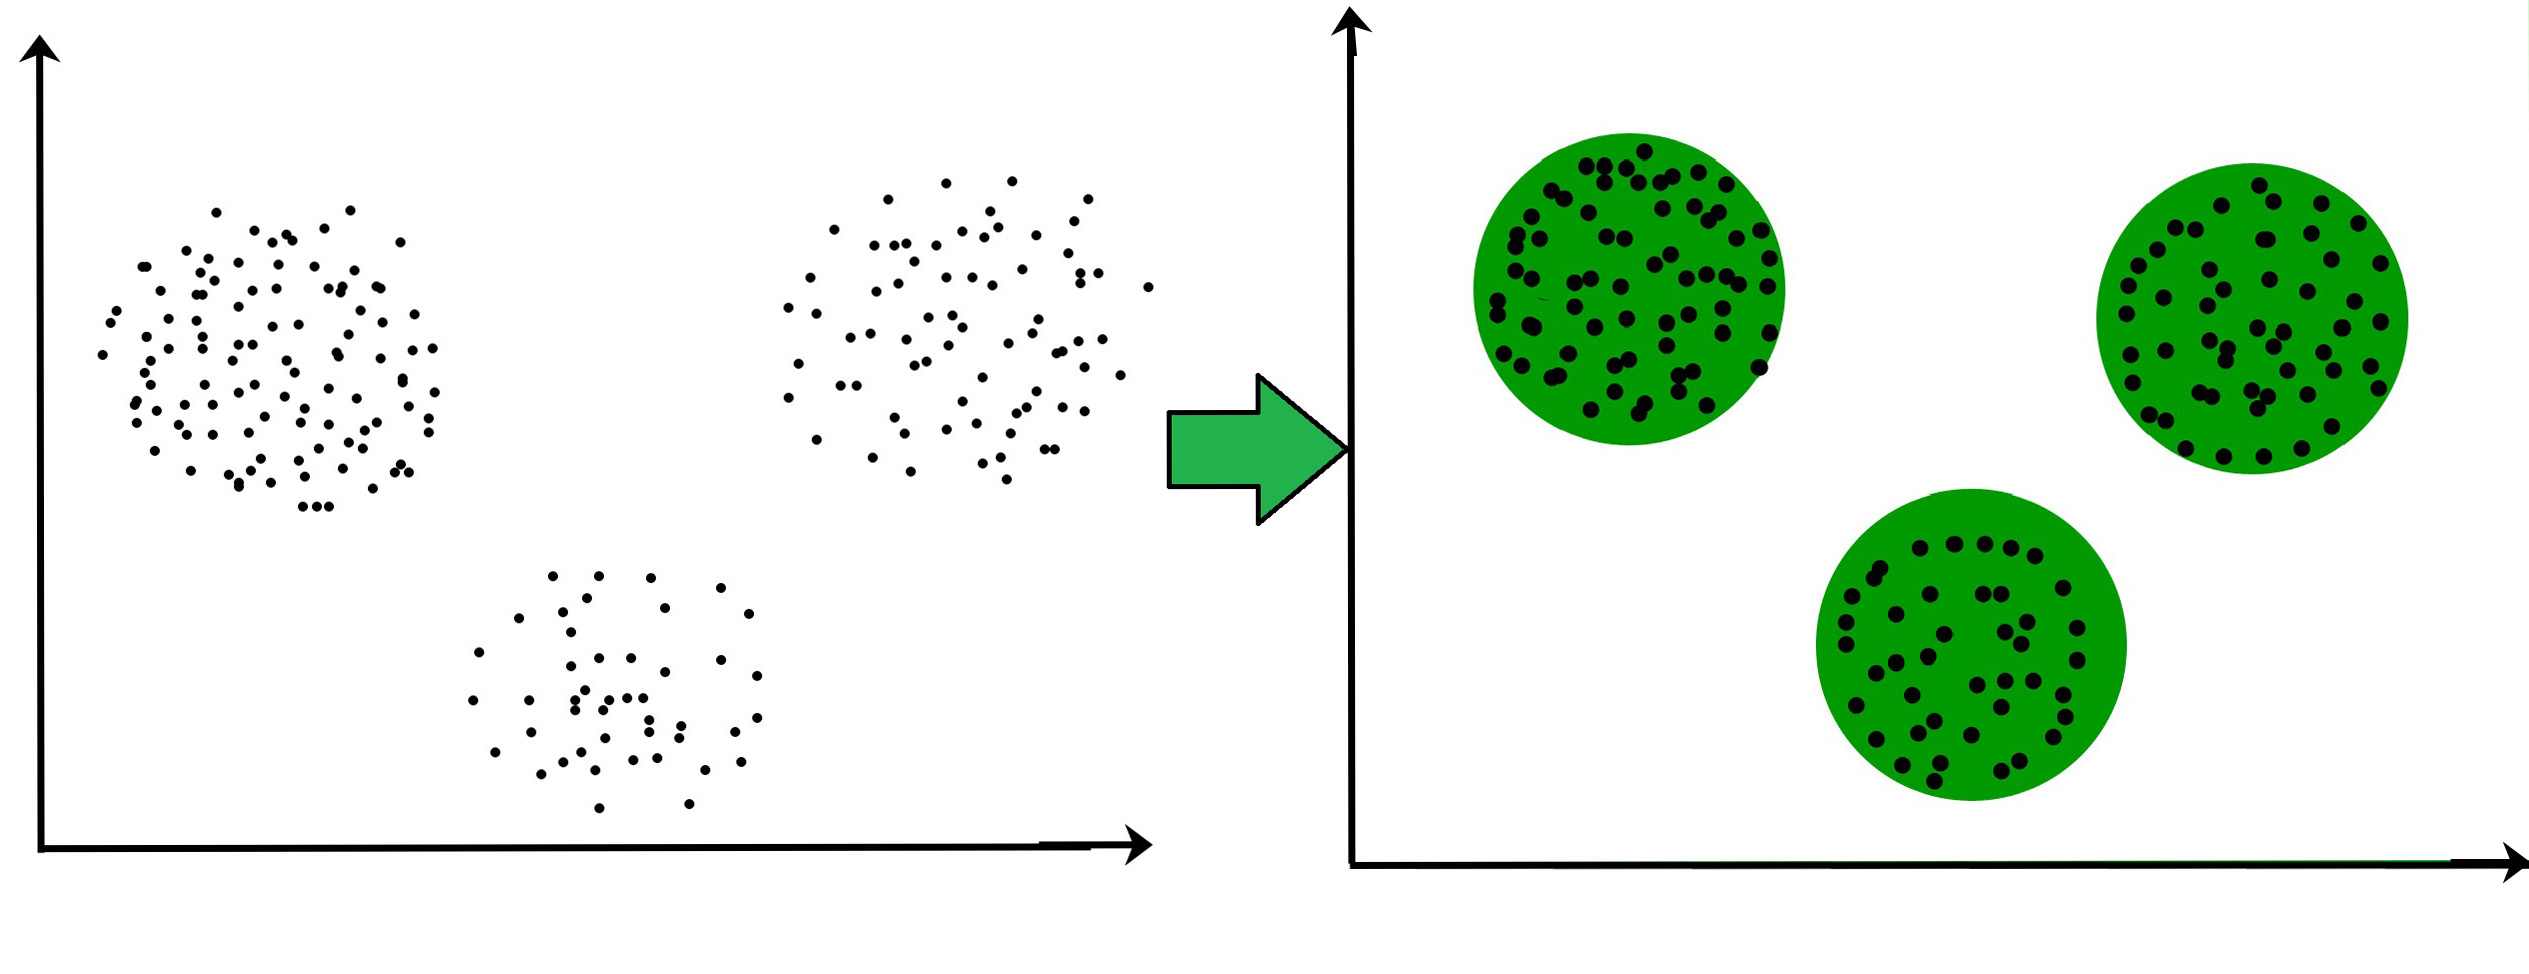
\includegraphics[width=0.7\textwidth]{images/clustering_intro.jpg}
    \caption{Γραφική αναπαράσταση ομαδοποίησης}
\end{figure}
\sloppy
Υπάρχουν εκατοντάδες αλγόριθμοι ομαδοποίησης οι οποίοι χρησιμοποιούν διαφορετικές μεθόδους και
τεχνικές. Δεν υπάρχει κάποιος που να υπερτερεί πλήρως των υπολοίπων αλλά η καταλληλότητα του Κάθε
αλγορίθμου εξαρτάται από το σύνολο δεδομένων. Παρά τις διαφορές τους μπορούμε να τους εντάξουμε σε
κατηγορίες συμφωνά με τον τρόπο που κάνουν την ομαδοποίηση. Οι τέσσερις πιο βασικές κατηγορίες
είναι:
\fussy
\begin{itemize}
    \item \textlatin{Centroid based clustering}
    \item \textlatin{Density based clustering}
    \item \textlatin{Distribution based clustering}
    \item \textlatin{Hierarchical clustering}
\end{itemize}
Οι κατηγορίες αυτές θα αναλυθούν περισσότερο στη συνέχεια. Επιπλέον, θα δούμε και τους πιο διάσημους αλγορίθμους που ανήκουν σε αυτές της κατηγορίες και θα αναλύσουμε και τον τρόπο
λειτουργίας τους.

\subsection{\textlatin{Centroid based clustering}}
Οι αλγόριθμοι τύπου \textlatin{Centroid based clustering} όπως μπορούμε να καταλάβουμε κάνουν ομαδοποίηση με βάση τα κέντρα. Αυτό σημαίνει ότι θα έχουμε τόσα κέντρα όσες και οι ομάδες που επιλέξαμε.
Έπειτα για να ομαδοποιήσουμε όλα τα σημεία του χώρου θα βλέπουμε σε ποιο κέντρο βρίσκονται πιο κοντά και θα τα εντάσσουμε στην ομάδα αυτού του κέντρου. Το πρόβλημα εδώ είναι πως θα βρούμε τα
κατάλληλα κέντρα. Αν δεν επιλέξουμε τα κέντρα σωστά τότε η ομαδοποίηση πυ θα κάνουμε θα απέχει πολύ από την πραγματικότητα. Γι' αυτό και οι συγκεκριμένοι αλγόριθμοι έχουν ως βασική δουλειά να
προσεγγίσουν αυτά τα κέντρα.\par Για να καταλάβουμε με ποιον τροπο συμβαίνει αυτό θα δούμε τον αλγόριθμο \textlatin{k-Means} που είναι και ο πιο διάσημος αλγόριθμος ταξινόμησης με βάση τα κέντρα.
Το \textlatin{k} είναι το πλήθος των ομάδων που θέλουμε. ξεκινάμε τον αλγόριθμο επιλέγοντας \textlatin{k} τυχαία κέντρα στον χώρο και χωρίζουμε τα υπόλοιπα σημεία σε ομάδες ανάλογά με την εγγύτητα
τους στα τυχαία κέντρα. Έτσι έχουμε καταλήξει σε μια αρχική προσέγγιση. Έπειτα θα βρούμε το πραγματικό κέντρο των ομάδων που δημιουργήθηκαν βρίσκοντας τη μέση τιμή των σημείων που ανήκουν στην
ομάδα. Αυτή η διαδικασία επαναλαμβάνεται και έτσι κάποια στιγμή τα τελικά κέντρα θα μπορούν να κάνουν καλή ομαδοποίηση.
\begin{figure}[H]
    \centering
    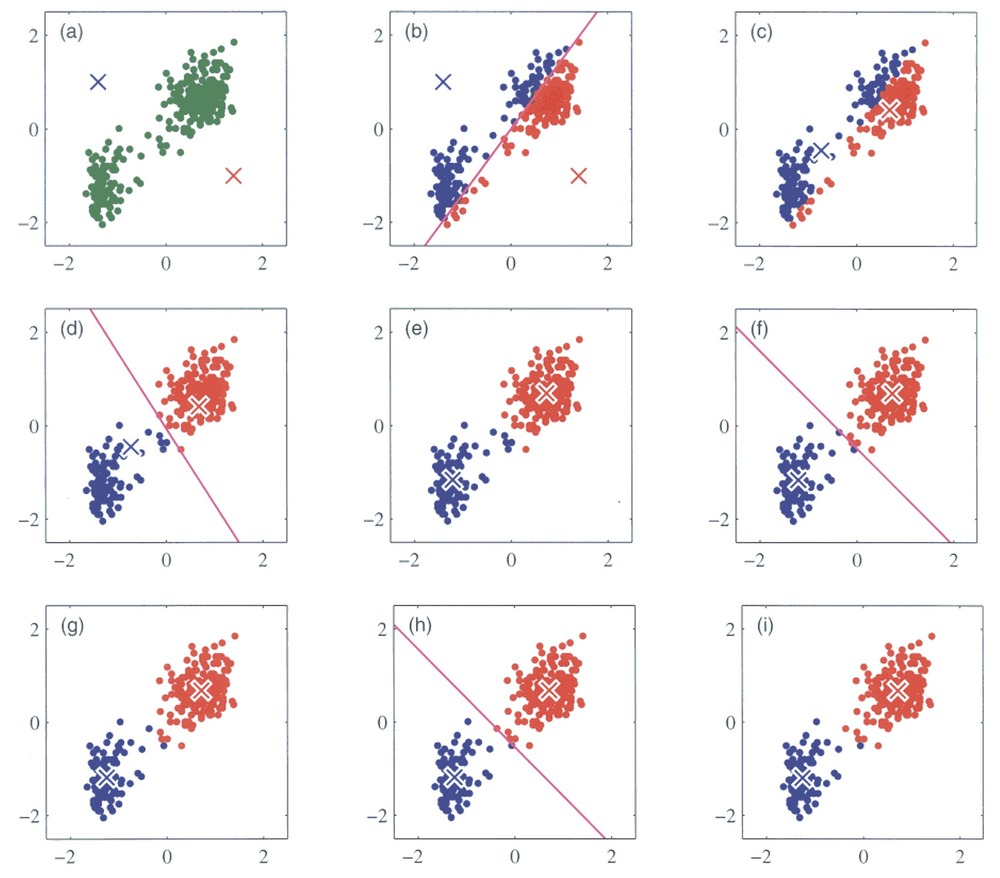
\includegraphics[width=1\textwidth]{images/kmeans.jpg}
    \caption{Επαναλήψεις του αλγορίθμου \textlatin{k-Means}}
\end{figure}
Ένα από τα πλεονεκτήματα του αλγορίθμου είναι η απλότητα του. Επιπλέον λειτουργεί καλά σε μεγάλο σύνολο δεδομένων και εξασφαλίζει ότι θα συγκλίνει σε κάποια λύση. Επίσης μπορεί αν δημιουργήσει
ομάδες διαφορετικού μεγέθους και σχήματος. Παρ' όλα αυτά τα αποτελέσματα τα τελικά αποτελέσματα του αλγορίθμου εξαρτώνται από τις αρχικές συνθηκες. Άρα εφόσον αρχικοποιούμε τα κέντρα τυχαία, αν
ξανά τρέξουμε τον αλγόριθμο θα πάρουμε διαφορετικά αποτελέσματα. Επίσης πρέπει να ορίσουμε μόνοι μας το πλήθος των ομάδων που είναι κάτι που μπορεί να μην θέλουμε πάντα\cite{kmeans1}.
\subsection{\textlatin{Density based clustering}}
\subsection{\textlatin{Distribution based clustering}}
\subsection{\textlatin{Hierarchical clustering}}